
%(BEGIN_QUESTION)
% Copyright 2007, Tony R. Kuphaldt, released under the Creative Commons Attribution License (v 1.0)
% This means you may do almost anything with this work of mine, so long as you give me proper credit

This PLC is being used to start and stop an electric motor, and also to shut it down automatically in the event of excessive vibration, overcurrent, or high motor winding temperature:

$$\includegraphics[width=15.5cm]{i02662x01.eps}$$

The status of each shutdown contact is as follows:

\begin{itemize}
\goodbreak
\item{} Vibration contact: {\it open} when good, {\it closes} when vibration becomes excessive
\item{} Overload contact: {\it closed} when good, {\it opens} when overloaded
\item{} Temperature contact: {\it closed} when good, {\it opens} when hot
\end{itemize}

Draw a PLC ladder-logic program to start and stop this motor.  Be sure to make the program latching so that the operator does not have to hold the Start button to keep the motor running.

$$
\includegraphics[width=15.5cm]{i02662x02.eps}$$

\vskip 20pt \vbox{\hrule \hbox{\strut \vrule{} {\bf Suggestions for Socratic discussion} \vrule} \hrule}

\begin{itemize}
\item{} A powerful problem-solving technique is to simplify the problem so that it is easier to solve, then use that solution as a starting point for the final solution of the given (complex) problem.  Show how you would first simplify the given problem here, and what that simple(r) solution would look like.
\item{} Explain how you could fool the PLC into ``thinking'' there was a high-temperature condition when in fact there was not.
\item{} Explain how you could fool the PLC into ``thinking'' there was a high-vibration condition when in fact there was not.
\item{} Explain how you could fool the PLC into ``thinking'' there was an overload condition at the motor when in fact there was not.
\end{itemize}

\underbar{file i02662}
%(END_QUESTION)





%(BEGIN_ANSWER)


%(END_ANSWER)





%(BEGIN_NOTES)

$$\includegraphics[width=15.5cm]{i02662x03.eps}$$

\vskip 20pt \vbox{\hrule \hbox{\strut \vrule{} {\bf Virtual Troubleshooting} \vrule} \hrule}

This question is a good candidate for a ``Virtual Troubleshooting'' exercise.  Presenting the diagram to students, you first imagine in your own mind a particular fault in the system.  Then, you present one or more symptoms of that fault (something noticeable by an operator or other user of the system).  Students then propose various diagnostic tests to perform on this system to identify the nature and location of the fault, as though they were technicians trying to troubleshoot the problem.  Your job is to tell them what the result(s) would be for each of the proposed diagnostic tests, documenting those results where all the students can see.

During and after the exercise, it is good to ask students follow-up questions such as:

\begin{itemize}
\item{} What does the result of the last diagnostic test tell you about the fault?
\item{} Suppose the results of the last diagnostic test were different.  What then would that result tell you about the fault?
\item{} Is the last diagnostic test the best one we could do?
\item{} What would be the ideal order of tests, to diagnose the problem in as few steps as possible?
\end{itemize}

%INDEX% PLC, programming challenge: motor shutdown control system

%(END_NOTES)


